\documentclass[aspectratio=169]{beamer}

% Pacotes essenciais
\usepackage[utf8]{inputenc}
\usepackage[T1]{fontenc}
\usepackage[brazilian]{babel}
\usepackage{graphicx}
\usepackage{tikz}
\usepackage{media9}
\usepackage{hyperref}

% Fonte moderna Roboto
\usepackage[sfdefault]{roboto}
\usepackage[T1]{fontenc}

% Definição das cores
\definecolor{vermelhoPrincipal}{HTML}{b11116}
\definecolor{azulComplementar}{HTML}{3a5461}
\definecolor{brancoFundo}{HTML}{FFFFFF}

% Configuração do tema
\usetheme{Madrid}
\usecolortheme{default}

% Cores personalizadas - texto sempre em preto
\setbeamercolor{structure}{fg=black}
\setbeamercolor{palette primary}{bg=vermelhoPrincipal,fg=white}
\setbeamercolor{palette secondary}{bg=azulComplementar,fg=white}
\setbeamercolor{palette tertiary}{bg=vermelhoPrincipal,fg=white}
\setbeamercolor{palette quaternary}{bg=azulComplementar,fg=white}
\setbeamercolor{frametitle}{bg=vermelhoPrincipal,fg=white}
\setbeamercolor{background canvas}{bg=brancoFundo}
\setbeamercolor{title}{fg=black}
\setbeamercolor{subtitle}{fg=azulComplementar}
\setbeamercolor{author}{fg=black}
\setbeamercolor{date}{fg=black}
\setbeamercolor{itemize item}{fg=black}
\setbeamercolor{itemize subitem}{fg=black}
\setbeamercolor{enumerate item}{fg=black}
\setbeamercolor{block title}{bg=vermelhoPrincipal,fg=white}
\setbeamercolor{block body}{bg=vermelhoPrincipal!10,fg=black}
\setbeamercolor{normal text}{fg=black}

% Configurar fonte dos itemize
\setbeamerfont{itemize/enumerate body}{size=\scriptsize}
\setbeamerfont{itemize/enumerate subbody}{size=\scriptsize}

% Marcadores modernos e minimalistas
\setbeamertemplate{itemize item}{\raisebox{0.2ex}{\rule{0.6ex}{0.6ex}}}
\setbeamertemplate{itemize subitem}{\raisebox{0.3ex}{\rule{0.4ex}{0.4ex}}}
\setbeamertemplate{itemize subsubitem}{\raisebox{0.35ex}{\rule{0.3ex}{0.3ex}}}
\setbeamertemplate{enumerate items}[square]

% Transições suaves
\setbeamercovered{transparent}

% Remover símbolos de navegação
\setbeamertemplate{navigation symbols}{}

% Customizar o cabeçalho com barra vermelha e logo
\setbeamertemplate{headline}{
  \begin{beamercolorbox}[wd=\paperwidth,ht=0.6cm,dp=0.15cm,leftskip=0.2cm,rightskip=0.4cm]{palette primary}
    \raisebox{-0.05cm}{
\includegraphics[height=0.45cm]{imgs/base/fatec-rgt.png}}
    \hfill
    \raisebox{-0.18cm}{
\includegraphics[height=0.85cm]{imgs/base/governo-sp-secretaria-logo.png}}
    \hspace{0.2cm}
    \raisebox{-0.08cm}{
\includegraphics[height=0.6cm]{imgs/base/cps-logo.png}}
  \end{beamercolorbox}
}
% Remover sombras dos blocks
\setbeamertemplate{blocks}[default]
\setbeamertemplate{itemize/enumerate body begin}{\scriptsize}
\setbeamertemplate{itemize/enumerate subbody begin}{\scriptsize}
% Customizar o rodapé
\setbeamertemplate{footline}{
  \begin{beamercolorbox}[wd=\paperwidth,ht=0.4cm,dp=0.2cm,leftskip=0.3cm,rightskip=0.3cm]{palette secondary}
    \usebeamerfont{footline}
    \insertshortauthor \hfill \hfill {\fontsize{5}{6}\selectfont\insertshorttitle} \hfill \hfill \insertframenumber/\inserttotalframenumber
  \end{beamercolorbox}
}

% Customizar título do frame
\setbeamertemplate{frametitle}{
  \vspace{0.3cm}
  \textcolor{black}{\insertframetitle}
  \vspace{0.1cm}
}

% Informações da apresentação
\title{Detecção de fungos parasitas em cogumelos por meio de Aprendizagem Profunda}
\subtitle{}
\author[DSM]{Barros, L.; Viana, E.; Andrei, L.; Estevam, R.; Sueoka, L.}
\institute{Desenvolvimento de Software Multiplataforma\\FATEC Registro}
\date{\today}

\begin{document}

% Slide de título moderno
\begin{frame}
  \vspace{0.8cm}
  \begin{center}
    \begin{tikzpicture}
      % Linha decorativa superior
      \draw[vermelhoPrincipal, line width=2pt] (-4,0) -- (4,0);
    \end{tikzpicture}
    
    \vspace{0.4cm}
    
    {\normalsize\bfseries\inserttitle}\par
    
    \vspace{0.2cm}
    
    {\tiny\insertauthor}\par
    
    \vspace{0.1cm}
    
    {\small\textcolor{azulComplementar}{\insertsubtitle}}\par
    
    \vspace{0.5cm}
    
    \begin{tikzpicture}
      % Linha decorativa inferior
      \draw[azulComplementar, line width=1.5pt] (-2.5,0) -- (2.5,0);
    \end{tikzpicture}
    
    \vspace{0.3cm}
    
    {\scriptsize\insertinstitute}\par
    
    \vspace{0.01cm}
    
    {\tiny\textcolor{azulComplementar}{\insertdate}}\par
  \end{center}
\end{frame}

% Slide de agenda
\begin{frame}[b]{Agenda}
  \begin{itemize}
    \item Pitch
    \item Problematização
    \item Estado da Arte
    \item Objetivo
    \item Ferramental
    \item Metodologia
    \item Apresentação prática
  \end{itemize}
  
  \vfill
  
  \hfill{\scriptsize \textbf{Duração:} 10 a 11 min.}
\end{frame}

\section{Pitch}
{
\begin{frame}{Pitch}

\begin{center}

\vspace{2cm}

\Huge \textbf{Pitch do Projeto}

\vspace{1cm}

\href{https://www.youtube.com/watch?v=zmXlzcdq65A}{
\beamerbutton{Assistir Vídeo}
}

\end{center}

\end{frame}
}


\section{Problematização}

\begin{frame}{Problematização}

\vspace{-0.3cm}

\begin{columns}[c]

% Texto
\begin{column}{0.55\textwidth}

\begin{itemize}

\item \parbox{0.95\linewidth}{
\textbf{Problema}: fungos parasitas, infecções e deformidades afetam a produção de cogumelos.
}

\vspace{0.05cm}

\item \parbox{0.95\linewidth}{
\textbf{Causas e Consequências}: monitoramento manual e detecção tardia geram perdas produtivas e financeiras.
}

\vspace{0.05cm}

\item \parbox{0.95\linewidth}{
\textbf{Público Alvo}: fungicultores impactados pela redução da qualidade e produtividade.
}

\vspace{0.05cm}

\item \parbox{0.95\linewidth}{
\textbf{Relevância}: uso de IA e IoT para monitoramento e detecção precoce de contaminações.
}

\vspace{0.05cm}

\item \parbox{0.95\linewidth}{
\textbf{Lacunas}: falta de soluções integradas para monitoramento, dados agrícolas e controle de infecções.
}

\end{itemize}

\end{column}

% Imagem
\begin{column}{0.50\textwidth}

\centering

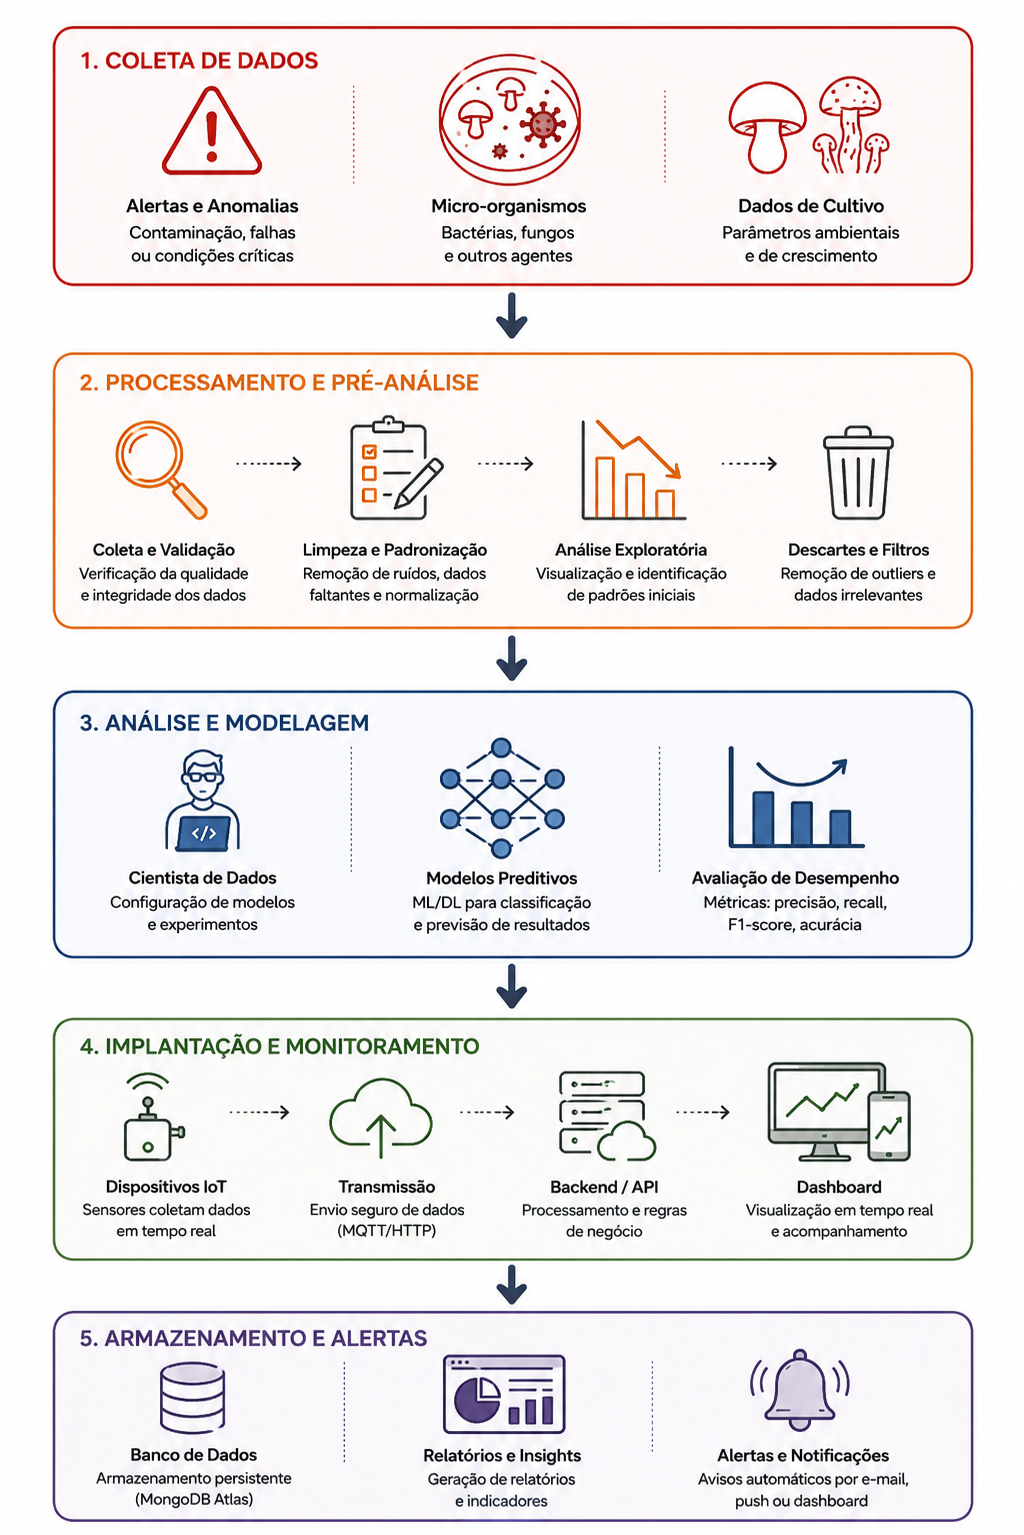
\includegraphics[
height=0.80\textheight,
keepaspectratio
]{imgs/diag.png}

{\tiny Fonte: Elaboração própria}

\end{column}

\end{columns}

\end{frame}


\section{Estado da Arte}

\begin{frame}[t]{Estado da Arte}
\scriptsize

Comparação de \textbf{soluções e pesquisas existentes} para monitoramento de cogumelos, destacando tecnologias utilizadas, resultados obtidos, limitações identificadas e lacunas exploradas pelo projeto Selene.

\vspace{0.3cm}

\begin{table}
\centering
\tiny

\resizebox{\textwidth}{!}{
\begin{tabular}{|p{2.8cm}|p{2.2cm}|p{2.2cm}|p{2.2cm}|p{2.2cm}|p{2cm}|}
\hline

\textbf{Título/Autores} &
\textbf{Objetivo} &
\textbf{Método} &
\textbf{Resultados} &
\textbf{Limitações} &
\textbf{Gap} \\
\hline

Moysiadis et al. (2023) &
Detectar, classificar e prever o crescimento de cogumelos. &
YOLOv5 e Detectron2 &
F1 de 76,5\% e acurácia de 70\% &
Dependência da qualidade das imagens e baixa detecção inicial. &
Sem IoT, alertas em tempo real e suporte a múltiplas espécies. \\
\hline

Rahman et al. (2022) &
Monitoramento remoto e classificação de cogumelos. &
IoT e Machine Learning &
Acurácia entre 90\% e 100\% &
Sem monitoramento visual e detecção de doenças. &
Ausência de visão computacional e reconhecimento de infecções. \\
\hline

Nuankaew et al. (2025) &
Detectar mofo verde em cogumelos ostra. &
CNN, IoT e aplicação web &
Acurácia de 92,5\% &
Dataset reduzido e influência de fatores ambientais. &
Sem gestão da produção e centralização de dados. \\
\hline

\end{tabular}
}

\end{table}

\end{frame}


\section{Objetivo}

\begin{frame}{Objetivo}

\begin{columns}[c]

% Texto
\begin{column}{0.58\textwidth}

\begin{itemize}

\item \parbox{0.95\linewidth}{
\textbf{Objetivo Geral}: desenvolver um sistema inteligente para monitoramento do cultivo de cogumelos com IA e IoT.
}

\vspace{0.05cm}

\item \textbf{Objetivos Específicos:}

{\footnotesize
\begin{itemize}

\item Detectar contaminações e deformidades.

\item Monitorar condições ambientais.

\item Centralizar dados do cultivo.

\item Emitir alertas automáticos.

\item Validar a solução com produtores.

\end{itemize}
}

\vspace{0.05cm}

\item \parbox{0.95\linewidth}{
\textbf{Resultados Esperados}: reduzir perdas e aumentar a produtividade.
}

\vspace{0.05cm}

\item \parbox{0.95\linewidth}{
\textbf{Métricas de Sucesso}: acurácia superior a 50\% e falsos positivos inferiores a 10\%.
}

\end{itemize}

\end{column}

% Imagem
\begin{column}{0.50\textwidth}

\centering

\hspace{-0.5cm}
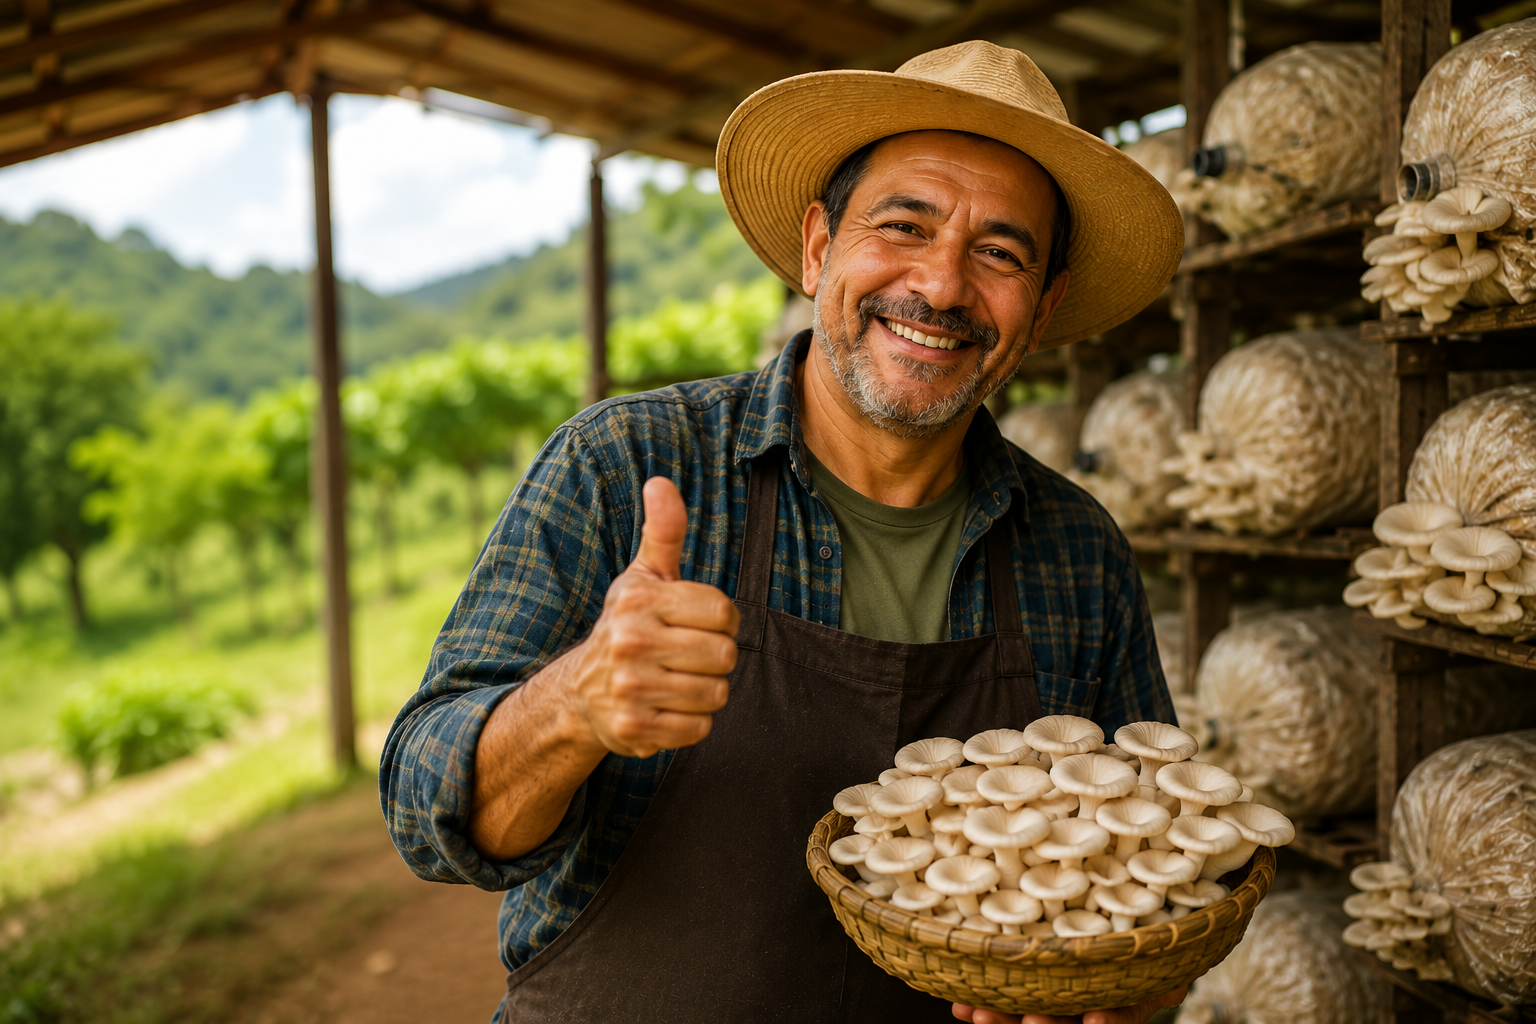
\includegraphics[
height=0.60\textheight,
keepaspectratio
]{imgs/objt.png}

\vspace{0.1cm}

{\tiny Fonte: Elaboração própria}

\end{column}

\end{columns}

\end{frame}


\section{Ferramental}

\begin{frame}{Ferramental}

\begin{columns}[c]

% Texto (ligeiramente menor para liberar espaço)
\begin{column}{0.48\textwidth}

\scriptsize

\begin{itemize}

\item \textbf{Controle de Versão}: Git, GitHub e GitHub Actions.
\item \textbf{Backend}: Node.js, Express, Socket.io e dotenv.
\item \textbf{Banco de Dados}: MongoDB Atlas e Mongoose.
\item \textbf{Mobile}: React Native, Expo e Expo Router.
\item \textbf{Integrações}: API REST, Axios, Cloudinary e Multer.
\item \textbf{Segurança}: JWT, OAuth 2.0, Helmet e CORS.
\item \textbf{Infraestrutura}: Docker, Rede Local (LAN) e Computação em Nuvem.
\item \textbf{Ferramentas}: Figma, AsyncStorage e módulos Expo.

\end{itemize}

\end{column}

% Imagem (maior)
\begin{column}{0.52\textwidth}

\centering

\hspace*{0.3cm}
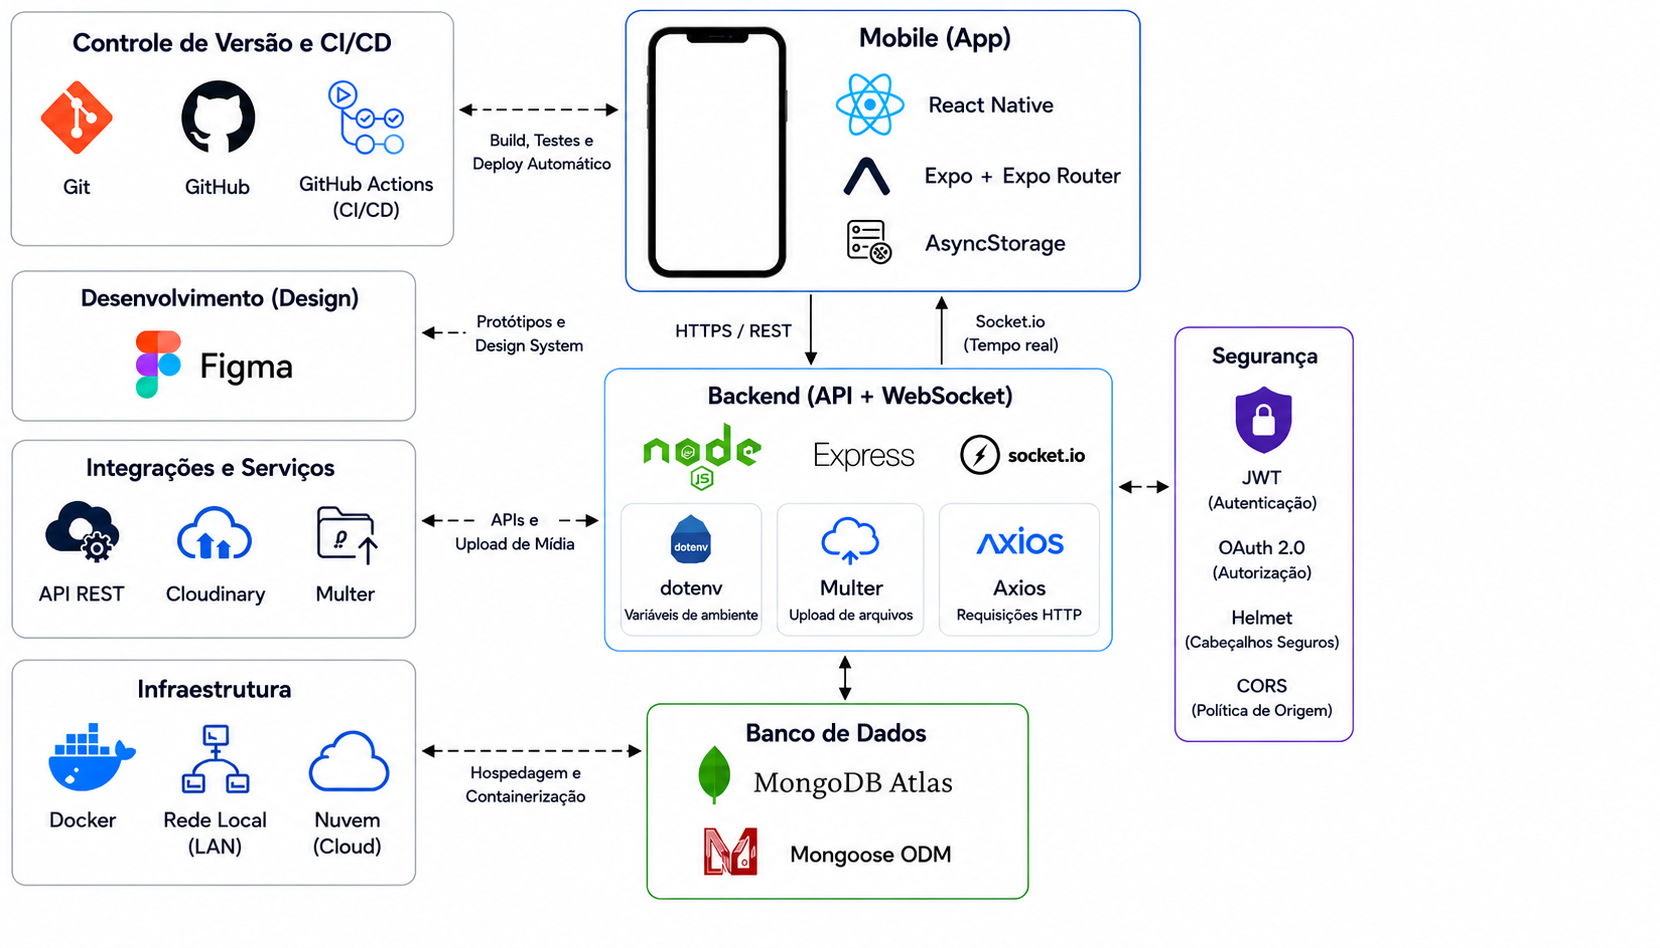
\includegraphics[
width=\linewidth,
height=0.88\textheight,
keepaspectratio
]{imgs/ferr.png}

\vspace{0.05cm}

{\tiny Fonte: Elaboração própria}

\end{column}

\end{columns}

\end{frame}


\section{Metodologia}

\begin{frame}[t]{Metodologia}

\scriptsize

\vspace{0.1cm}

\centering
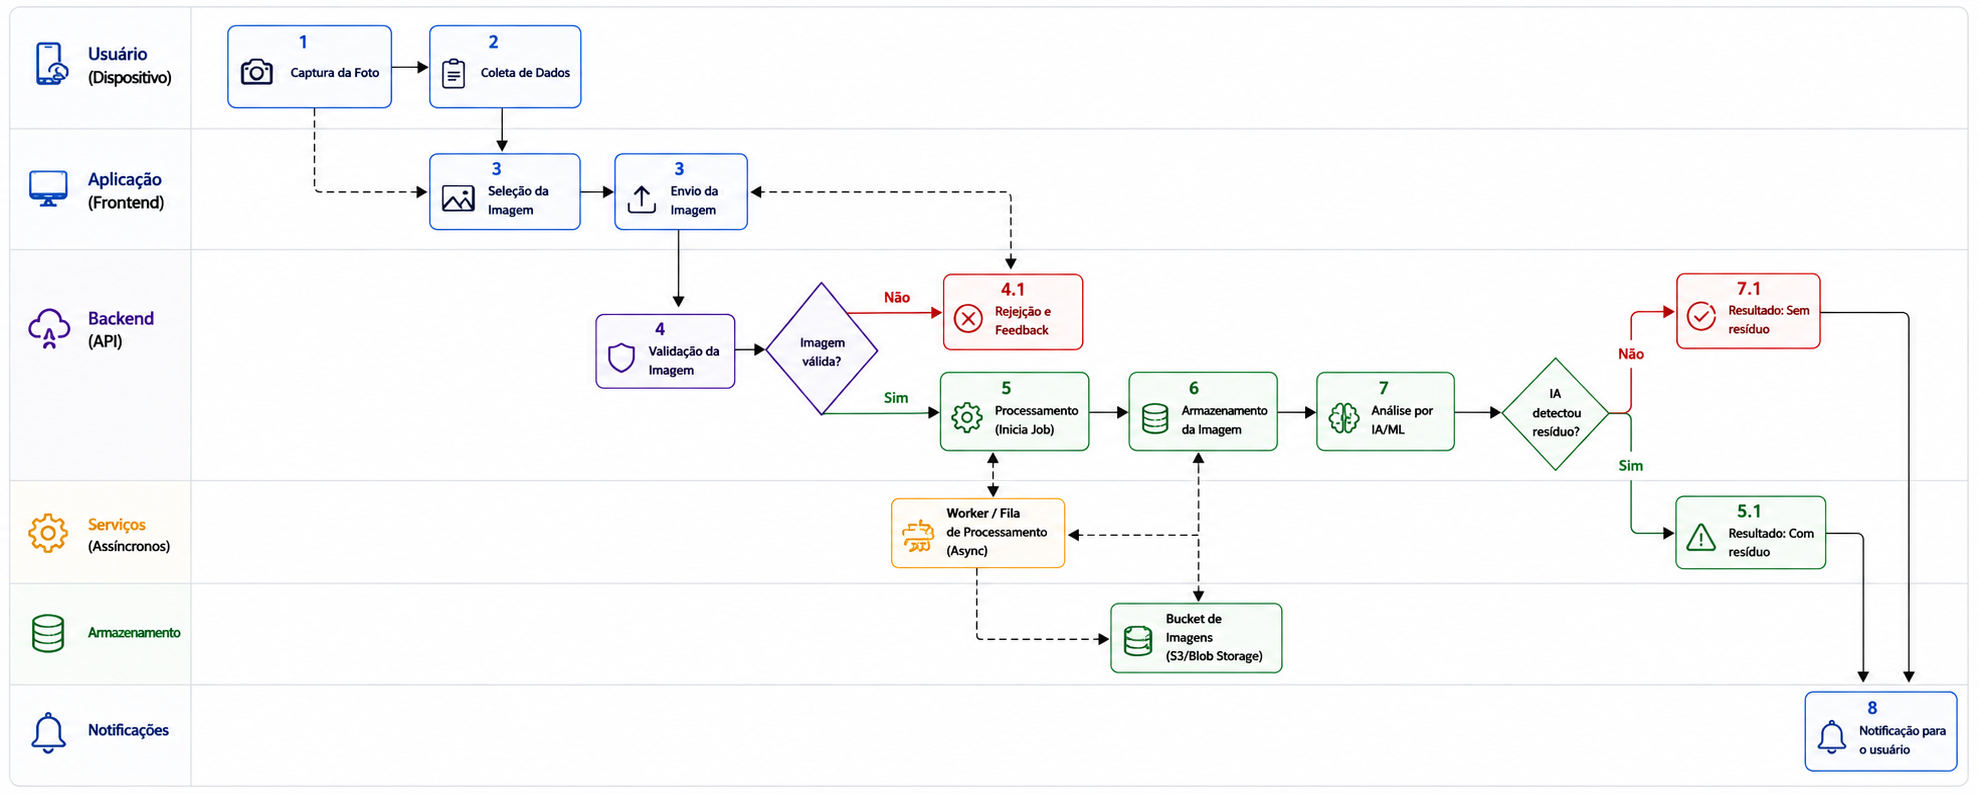
\includegraphics[
    width=\textwidth,
    height=0.75\textheight,
    keepaspectratio
]{imgs/met.png}

\end{frame}


\begin{frame}{Apresentação Prática}

\begin{columns}[T]

% Coluna da esquerda (texto)
\begin{column}{0.55\textwidth}
\begin{itemize}
    \item \textbf{Demonstração} do aplicativo de monitoramento do cultivo.
    \item Visualização em tempo real dos dados de produção.
    \item Fluxo completo de monitoramento, análise e \textbf{tomada de decisão} do produtor.
\end{itemize}
\end{column}

% Coluna da direita (imagem)
\begin{column}{0.45\textwidth}
\centering
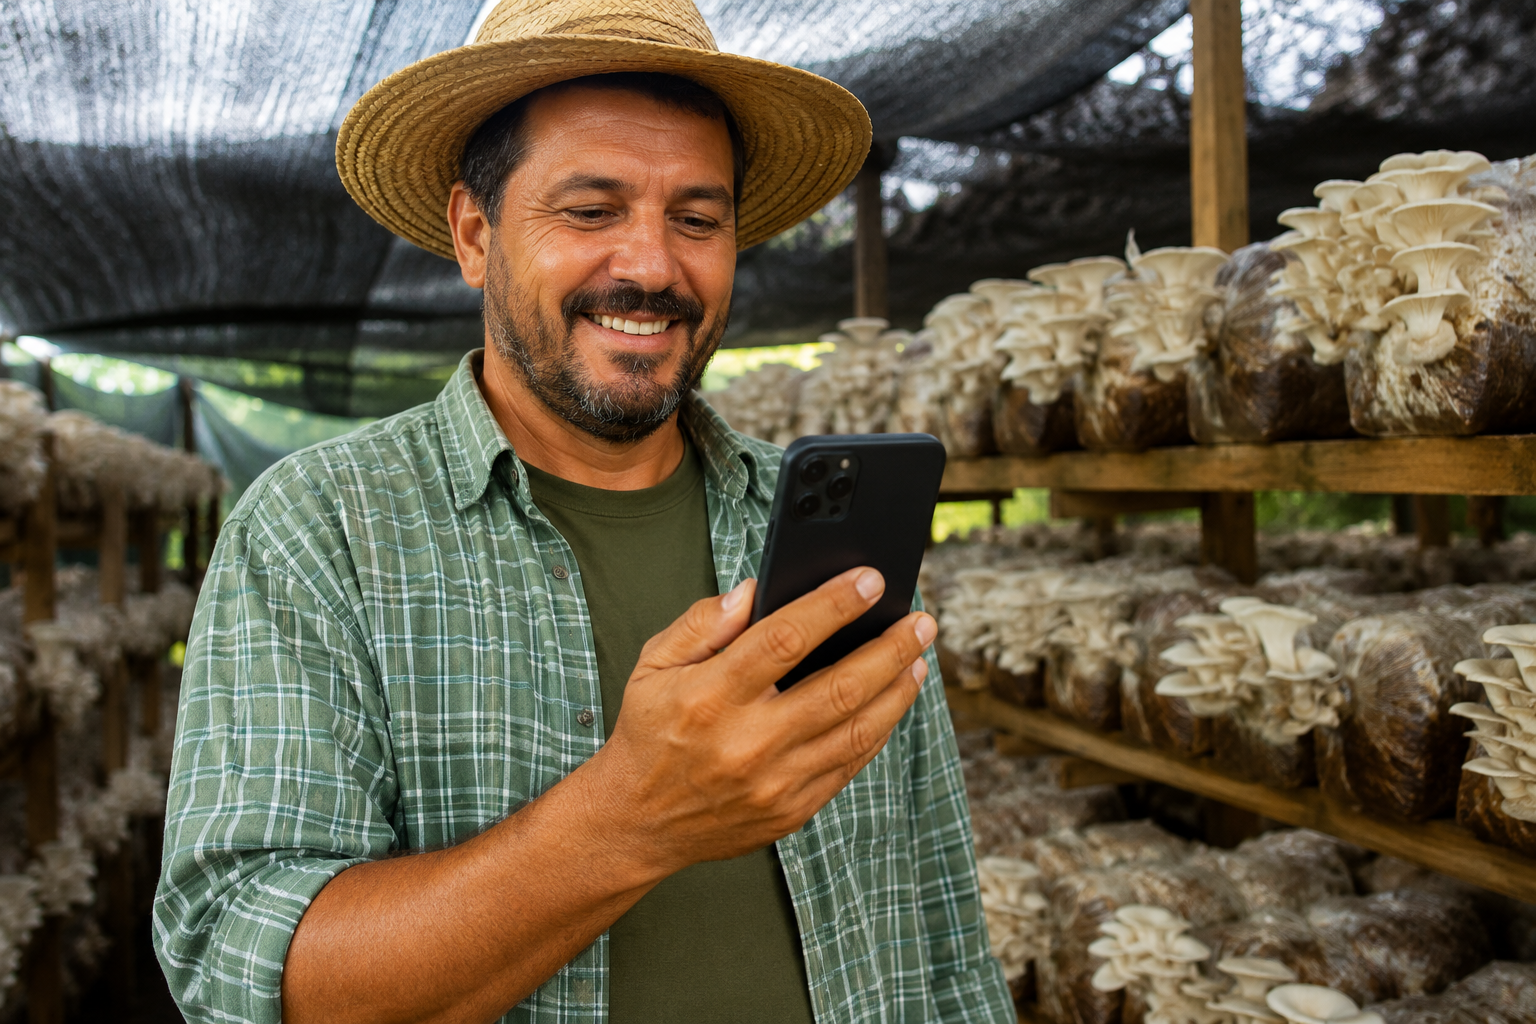
\includegraphics[width=\linewidth]{imgs/prat.png}
\end{column}

\end{columns}

\vfill

{\fontsize{4}{5}\selectfont
\textit{Fonte: Elaboração própria}
\hfill
}

\end{frame}


\begin{frame}
    \centering
    \Huge \textbf{Obrigado pela atenção!}
\end{frame}

\end{document}
